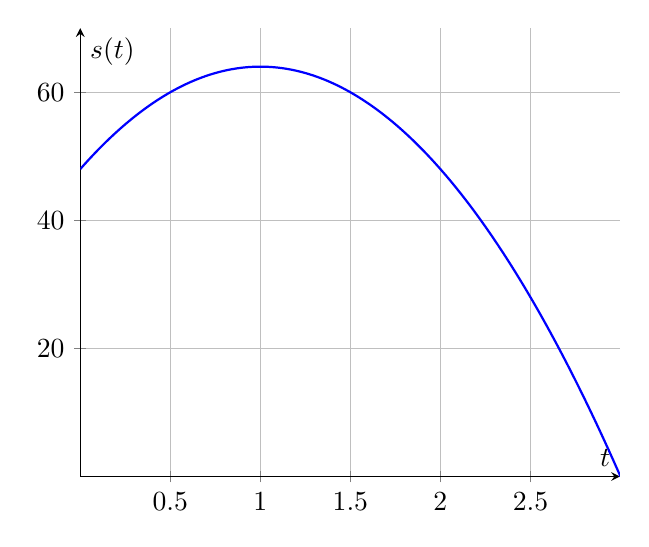
\begin{tikzpicture}[scale=1]
    \begin{axis}[
        samples = 900,
        axis lines=middle,
        grid=major,
     %  xmin=0, xmax=4,
       ymin=0, ymax=70,
       % xtick={0,0.5,...,4},
      % ytick={-2,-1,...,10},
      %	tick style={thick},
    % 	x label style={at={(axis description cs:1,0.7)}},
    % 	y label style={at={(axis description cs:0.4,1)}},
        ylabel=$s(t)$,
        xlabel=$t$,
            ]
        \addplot[domain=0:3, blue,  thick] {-16*x^2+32*x+48};
    \end{axis}
    \end{tikzpicture}